\documentclass[12pt]{article}

\usepackage{sbc-template}
\usepackage[utf8]{inputenc}
\usepackage[T1]{fontenc}
\usepackage{amsmath,amssymb}
\usepackage{graphicx}
\usepackage{booktabs}
\usepackage{url}
\usepackage{microtype}

\title{UM SISTEMA DE CONTROLE APRENDIDO PARA REDES QUÂNTICAS:\\
ROTEAMENTO, TEMPORIZAÇÃO DE REPETIDOR, COMPENSAÇÃO DE POLARIZAÇÃO\\
E BLOCAGEM DE CHAVE SOBRE UM SIMULADOR DE EVENTOS DISCRETOS}

\author{Alexandre O. S. Santos\textsuperscript{1,2}}

\begin{document}

\maketitle

\address{\textsuperscript{1}Quantum Industrial Innovation -- QuIIN\\
Senai CIMATEC -- Salvador, BA -- Brazil
\nextinstitute
\textsuperscript{2}Latin America Quantum Computing Center -- LAQCC\\
Senai CIMATEC -- Salvador, BA -- Brazil}

\email{alexandreoliversan1@gmail.com, alexandre.ssantos@fbter.org.br}

\begin{abstract}
This paper presents \texttt{qnet\_autopilot}, a learned control system for
quantum networks covering four decisions that are usually studied separately:
which links to entangle and in what order to swap them; when to purify and when
to swap rather than firing at a fixed threshold; how to predict and cancel
polarisation drift in real time; and how to split one fibre between classical
traffic and key distribution. All four are built on a closed-form physics layer
transcribed from, and checked against, the SeQUeNCe discrete-event simulator,
and are trained and scored on held-out seeds. The polarisation compensator
reaches a mean QBER of 0.0074 against 0.0383 for a per-operating-point retuned
alpha-beta filter, under an explicit hardware condition: an actuator faster
than 250 rad/s, below 120 rad/s the classical filter wins. The predictive
allocator delivers 2.7 times the classical throughput of static admission at
matched key service, and the ordering survives finite-key accounting. The
system's strongest single result is a causal, tuning-free key-block controller
that decides where to cut blocks from the same binomial estimates a receiver
publishes for parameter estimation: on a poorly compensated link it yields
4075 bit/s where no timer of any duration yields a single bit, reaching 95\% of
an exact dynamic-programming oracle by assembling one privacy-amplification
block out of roughly 29 disjoint windows. Two results are negative and
reported as such: with the heralding cost measured inside the event loop the
routing agent only ties the best heuristic, and no single compensator covers
45--180 Hz. The package ships with 861 tests.
\end{abstract}

\keywords{Keywords}{Quantum Networks, Entanglement Routing, Polarisation
Compensation, Finite-Key Analysis, Reinforcement Learning, Discrete-Event
Simulation}

\begin{resumo}
Este artigo apresenta o \texttt{qnet\_autopilot}, um sistema de controle
aprendido para redes quânticas que cobre quatro decisões normalmente estudadas
em separado: em quais enlaces gerar emaranhamento e em que ordem trocá-lo;
quando purificar e quando trocar, em vez de disparar num limiar fixo; como
prever e cancelar a deriva de polarização em tempo real; e como repartir uma
fibra entre tráfego clássico e distribuição de chaves. As quatro são
construídas sobre uma camada de física em forma fechada transcrita do simulador
de eventos discretos SeQUeNCe e conferida contra ele, e são treinadas e
avaliadas em sementes retidas. O compensador de polarização atinge QBER média
de 0,0074 contra 0,0383 do filtro alfa-beta ressintonizado em cada ponto de
operação, sob uma condição de hardware explícita: atuador acima de 250 rad/s,
sendo que abaixo de 120 rad/s o filtro clássico ganha. O alocador preditivo
entrega 2,7 vezes a vazão clássica da admissão estática a serviço de chave
igualado, e a ordenação sobrevive à contabilidade de chave finita. O resultado
mais forte do sistema é um controlador causal de bloco de chave, sem constante
de ajuste, que decide onde cortar os blocos a partir das mesmas estimativas
binomiais que um receptor publica para estimação de parâmetro: num enlace mal
compensado ele entrega 4075 bit/s onde nenhum temporizador de qualquer duração
entrega um único bit, atingindo 95\% de um oráculo exato de programação
dinâmica ao montar um bloco de amplificação de privacidade a partir de cerca de
29 janelas disjuntas. Dois resultados são negativos e reportados como tais: com
o custo de heralding medido dentro do laço de eventos, o agente de roteamento
apenas empata com a melhor heurística, e nenhum compensador único cobre a faixa
de 45 a 180 Hz. O pacote acompanha 861 testes.
\end{resumo}

\keywords{Palavras-chave}{Redes Quânticas, Roteamento de Emaranhamento,
Compensação de Polarização, Chave Finita, Aprendizado por Reforço, Simulação de
Eventos Discretos}

% ---------------------------------------------------------------------------
\section{Introdução}

Operar uma rede quântica é, do ponto de vista de controle, decidir
continuamente o que fazer com um recurso que se degrada sozinho. Pares
emaranhados distribuídos por fibra perdem fidelidade por decoerência de memória
e por flutuação de polarização induzida pelo ambiente termomecânico, e as
primitivas disponíveis para recuperá-los --- purificação de emaranhamento
\cite{bennett1996,deutsch1996} e troca de emaranhamento em cascata
\cite{briegel1998} --- consomem pares, tempo e ciclos de porta. Nós de repetidor
com interface em comprimento de onda de telecomunicações já foram demonstrados
em plataforma de íons aprisionados \cite{krutyanskiy2023}, o que desloca boa
parte da pergunta do domínio dos princípios para o domínio das decisões: quando
gerar, quando purificar, quando trocar, quando entregar, quando desistir.

Este artigo apresenta o \texttt{qnet\_autopilot}, um sistema de controle
aprendido que cobre quatro dessas decisões num único pacote, construído sobre o
simulador de eventos discretos SeQUeNCe \cite{wu2021}:

\begin{enumerate}
\item \textbf{Roteamento e temporização de repetidor}, formulados não como dois
  problemas mas como um único processo de decisão de Markov sobre as primitivas
  de rede, resolvido por uma política ator-crítico.
\item \textbf{Compensação de polarização em tempo real}, formulada como
  predição de rotação num horizonte de uma latência de controle à frente, a
  partir de estimativas ruidosas obtidas de fótons de monitoramento.
\item \textbf{Alocação híbrida clássico-quântica}, formulada como admissão: que
  fração da fibra liberar para tráfego clássico sabendo que o espalhamento
  Raman induzido eleva a QBER do canal quântico.
\item \textbf{Blocagem de chave de duração variável}, formulada como escolha
  das fronteiras dos blocos de amplificação de privacidade, resolvida por um
  controlador causal contra um oráculo exato.
\end{enumerate}

As quatro compartilham a mesma camada de física: uma transcrição em forma
fechada das rotinas de estado Bell-diagonal do SeQUeNCe, necessária porque
treinar exige milhares de episódios e um simulador de eventos discretos completo
é lento demais para isso, e conferida contra o simulador operação a operação,
trajetória a trajetória e, por fim, dentro do próprio laço de eventos.

Três decisões de método atravessam o trabalho e determinam o que os números
significam. Primeira: \emph{nenhum controlador vê a verdade}. O compensador
recebe uma amostra binomial finita de fótons de monitoramento, nunca a rotação
verdadeira; o controlador de bloco recebe os bits que o protocolo publica para
estimação de parâmetro, nunca a série de erro. Ambos são pontuados sobre a
verdade que nunca viram. Segunda: \emph{todo baseline é ressintonizado}. O
filtro alfa-beta é re-otimizado por busca em grade em cada ponto de operação, e
comparações pareadas por requisição substituem médias não pareadas onde a
variância entre tarefas domina. Terceira: \emph{resultados negativos são
reportados}. Dois dos quatro controladores não batem a alternativa simples, e
as seções que os descrevem dizem isso.

% ---------------------------------------------------------------------------
\section{Trabalhos Relacionados}

\subsection{Aprendizado aplicado a repetidores e roteamento}

O uso de aprendizado por reforço para descobrir e otimizar protocolos de
comunicação quântica foi estabelecido por \cite{wallnofer2020}, que mostra um
agente redescobrindo teleportação, purificação e esquemas de repetidor por
simulação projetiva. Para roteamento, \cite{roik2024} aplica aprendizado por
reforço à escolha de rotas em redes de comunicação quântica e \cite{le2022}
formula o roteamento de emaranhamento como problema de aprendizado por reforço
profundo. Para destilação, \cite{krastanov2019} busca circuitos de purificação
por algoritmo genético e \cite{chittoor2023} otimiza circuitos parametrizados
para destilação sob operações locais e comunicação clássica ruidosa.

O sistema descrito aqui difere desse conjunto em dois pontos. O espaço de ação
inclui \textsc{esperar} e \textsc{descartar} além das primitivas produtivas, de
modo que a política pode escolher \emph{não} agir --- e a Seção 7.2 mostra que
essa escolha importa. E o custo temporal de cada primitiva não é herdado do
modelo analítico: é medido contra o protocolo do simulador, o que muda o
resultado.

\subsection{Compensação de polarização}

O controle de polarização sem fim por cascata de retardadores é um resultado
clássico da óptica coerente \cite{noe1988} e continua sendo a base do hardware
de compensação. A literatura recente de controle em tempo real é dominada por
otimização clássica e não por aprendizado: \cite{young2026} compara descida de
gradiente, descida por coordenadas, recozimento simulado e algoritmos genéticos
para controle eletrônico de polarização em QKD. Onde aprendizado aparece em
enlaces implantados, aparece tipicamente sobre deriva de \emph{fase} ---
\cite{zhang2021} usa uma rede recorrente de duas camadas para prever deriva de
referencial em 100 e 250 km de fibra. As oportunidades de sensoriamento e
comunicação integrados por aprendizado em polarização são revisadas em
\cite{rode2025}. O compensador da Seção 5.2 é, portanto, comparado contra o
filtro clássico ressintonizado, que é o estado da prática, e não contra outro
modelo aprendido.

\subsection{Estatística de fibra instalada}

Não existe conjunto público de séries temporais de polarização em fibra
terrestre instalada; as séries baixáveis são submarinas e amostradas abaixo de
20 Hz, suficientes para deriva térmica e inúteis para a banda mecânica. As três
melhores caracterizações de enlaces terrestres publicam estatísticas e retêm os
dados: \cite{peterson2004} mede polarimetria Stokes a 4 kHz em 220 km de cabo
para-raios óptico e reporta um tom forte na frequência da rede elétrica com
harmônicos em 120 e 180 Hz; \cite{ramaswamy2026} caracteriza 15 km de cabo
aéreo/enterrado ao longo de 11 meses e reporta densidade espectral de deriva do
tipo \emph{flicker} com $\beta = 1{,}0 \pm 0{,}2$; \cite{shi2026} distribui
emaranhamento por 62 km com cerca de 70\% de trecho aéreo, com polarização
estável por dezenas de minutos à noite e movendo-se dezenas de graus em segundos
durante o dia. A escala da deriva lenta em fibra enterrada é fixada pela largura
de linha de polarização de \cite{czegledi2016}. O modelo de fibra da Seção 4.2 é
parametrizado por essas estatísticas.

\subsection{Coexistência clássico-quântica}

Sinais clássicos intensos na mesma fibra injetam ruído por espalhamento Raman
espontâneo, cujo coeficiente foi medido entre $1{,}5\times10^{-9}$ e
$3{,}1\times10^{-9}$ km$^{-1}$nm$^{-1}$ na banda C \cite{kumar2015}; os limites
de multiplexação em ambiente reconfigurável estão em
\cite{peters2009,chapuran2009} e a taxa alcançável com criptografia clássica de
1 Gbit/s na mesma fibra em \cite{eraerds2010}. Em operação metropolitana
contínua, \cite{dynes2019} reporta 580 dias de três enlaces de 5,0 a 10,6 km
com QBER entre 2,4\% e 2,7\%, sendo o incremento atribuível a um canal DWDM de
100 Gbit/s. Esses números fixam o acoplamento usado pelo alocador da
Seção 5.3.

% ---------------------------------------------------------------------------
\section{O Substrato Físico}

\subsection{Estados Bell-diagonais e as primitivas}

Pares emaranhados são representados como estados Bell-diagonais,
$\rho = \sum_i c_i |\beta_i\rangle\langle\beta_i|$, com
$(c_I, c_X, c_Y, c_Z)$ as populações nas quatro bases de Bell; o estado de
Werner \cite{werner1989} é o caso isotrópico. A escolha não é de conveniência:
é o formalismo do SeQUeNCe, e as transcrições mantêm os nomes de variável e as
assinaturas do simulador (\texttt{gate\_fid}, \texttt{meas\_fid},
\texttt{p\_succ}, \texttt{c\_I}/\texttt{c\_X}/\texttt{c\_Y}/\texttt{c\_Z}) para
que as duas implementações possam ser lidas lado a lado e qualquer divergência
apareça de imediato.

Sobre esse formalismo operam três primitivas. A purificação por recorrência
BBPSSW \cite{bennett1996} é definida sobre estados de Werner e devolve um
estado de Werner; DEJMPS \cite{deutsch1996} preserva a estrutura Bell-diagonal
completa. A troca de emaranhamento compõe dois pares numa medição de Bell, com
o limite analítico de Werner
$F_{out} = F_1F_2 + \frac{(1-F_1)(1-F_2)}{3}$. A geração é
\emph{single-heralded}: o formalismo Bell-diagonal não sabe escrever um fóton
isolado e portanto não representa a interferência de dois fótons de
Barrett--Kok \cite{barrett2005} --- uma restrição do formalismo, não uma
escolha, e a razão pela qual a comparação direta entre os dois simuladores é
possível.

\subsection{O modelo de fibra}

A fibra aplica ao estado de polarização uma rotação $R(t) \in SO(3)$ no espaço
de Stokes, composta de três termos: deriva térmica lenta como processo de
Ornstein--Uhlenbeck \cite{uhlenbeck1930}, uma banda mecânica de tons com
harmônicos, e saltos discretos. Os três são parametrizados pelas estatísticas
de campo da Seção 2.3 e não por escolha de plausibilidade; a Seção 7.4 relata o
que aconteceu quando essa substituição foi feita.

\subsection{Chave secreta com bloco finito}

Toda taxa de chave é avaliada contra o limite composável de chave finita de
\cite{tomamichel2012}, com a fração de teste otimizada:

\begin{equation}
\ell \le n\left[1 - h(e + \mu)\right] - \mathrm{leak}_{EC}
        - \log_2\frac{2}{\varepsilon_{\mathrm{cor}}}
        - 2\log_2\frac{1}{2\varepsilon_{\mathrm{sec}}},
\quad
\mu = \sqrt{\frac{(n+k)(k+1)}{n k^2}\ln\frac{1}{\varepsilon_{\mathrm{sec}}}},
\end{equation}

com $n$ os bits reservados à chave e $k$ os gastos na estimativa do erro. Fixar
a fração de teste erra o limite silenciosamente --- mantê-la em 10\% faz o
limite convergir para 90\% do assintótico em vez de para ele; buscá-la
reproduz a taxa assintótica a uma fração de por cento em $10^{10}$ bits, e essa
convergência é a verificação de que o limite está certo.

Uma consequência de (1) organiza a Seção 5.4 e não aparece na fórmula
assintótica: \textbf{a chave de um bloco depende apenas do número de bits e da
sua taxa média de erro}. Um trecho de fibra ruim, portanto, envenena cada bit
que divide o bloco com ele; e, simetricamente, a chave de um bloco \emph{não
depende de quando os bits chegaram} --- a amplificação de privacidade roda sobre
um conjunto de bits peneirados, e nada no limite exige que sejam consecutivos.

% ---------------------------------------------------------------------------
\section{Arquitetura do Sistema}

O pacote é organizado em quatro camadas. A camada de física reimplementa as
rotinas de estado do simulador. A camada de ambiente expõe um processo de
decisão de Markov sobre essas rotinas, com espaço de ações
\{\textsc{gerar}, \textsc{purificar}, \textsc{trocar}, \textsc{entregar},
\textsc{descartar}, \textsc{esperar}\}. A camada de agentes contém as
heurísticas de referência e as políticas aprendidas, todas atrás de uma mesma
interface de duas funções, de modo que trocar a implementação de rede neural
não toca no ambiente, nos baselines nem na avaliação. A camada de validação
contém o mecanismo que reconstrói o estado do ambiente a partir de objetos do
simulador, e os relatórios.

\subsection{O que cada controlador tem permissão de saber}

Um compensador de polarização é excepcionalmente fácil de avaliar de forma
desonesta: o simulador guarda a rotação verdadeira, e alimentá-la em qualquer
ponto --- como \emph{feature}, como alvo de treino ou como referência da
correção --- produz um controlador excelente fora de linha e impossível de
implantar. O pacote impõe três barreiras, cada uma coberta por teste: colunas
de verdade de referência ficam num espaço de nomes \texttt{true\_*} e a
construção de janelas supervisionadas levanta erro se uma delas for passada
como característica; o alvo de treino é uma \emph{medição futura}, não a
verdade futura; e a correção em vigor em qualquer instante foi computada a
partir de dados com pelo menos uma latência de controle de idade. O
particionamento treino/teste é cronológico e com intervalo de guarda, porque
janelas sobrepostas embaralhadas tornam qualquer métrica de teste sem sentido.

% ---------------------------------------------------------------------------
\section{As Quatro Capacidades}

\subsection{Roteamento e temporização como um único MDP}

Roteamento e temporização não são tratados como problemas distintos. O estado é
descrito por 11 características globais --- fração do prazo restante, progresso
na entrega, pares vivos, fidelidade média e melhor, pressão de memória média e
máxima, alcance e cobertura do caminho de referência, limiar da requisição e
fração do orçamento de passos consumida --- e cada ação legal por 23
características, entre elas a probabilidade de heralding do enlace, o número
esperado de rodadas, a fidelidade prevista do resultado em forma fechada, o
ganho de fidelidade, a idade do par mais antigo, se o resultado conecta os
extremos da requisição e se o segmento do caminho ainda está descoberto.

A recompensa paga uma entrega qualificada mais um bônus proporcional à margem
de fidelidade, e cobra um custo de tempo proporcional à fração do prazo
consumida e um custo fixo por tentativa de geração. A política é um
ator-crítico com GAE($\lambda$) \cite{schulman2016}, bônus de entropia
decrescente e \emph{clipping} de gradiente, no espírito dos métodos de vantagem
\cite{mnih2016}, implementado em numpy com retropropagação manual conferida
contra diferenças finitas a $10^{-10}$. O treino usa modelagem de recompensa
baseada em potencial \cite{ng1999}, que deixa a política ótima inalterada, e a
avaliação sempre reporta o resultado \emph{não} modelado.

\subsection{O compensador de polarização}

O compensador recebe uma janela de estimativas de rotação recentes, expressas
como incrementos relativos ao instante atual --- o que torna o problema
invariante a translação na esfera de Poincaré e dispensa o modelo de reaprender
a restrição de $SO(3)$ --- e prevê a rotação uma latência de controle à frente.
Três famílias são comparadas no mesmo laço fechado: persistência, filtro
alfa-beta ressintonizado por busca em grade em \emph{cada} ponto de operação, e
preditores ajustados (regressão \emph{ridge}, que é o preditor de Wiener para
um processo gaussiano estacionário, e um perceptron multicamadas).

O comando previsto é convertido em ângulos de elemento por decomposição de
Euler sobre uma cascata de retardadores X-Y-X com curso finito, velocidade
finita e reset sem fim \cite{noe1988}, de modo que a avaliação inclui o custo
de mover o atuador e não apenas o de acertar a predição.

\subsection{O alocador híbrido}

A alocação é admissão: a cada instante, que fração da fibra liberar para
tráfego clássico, sabendo que o ruído Raman induzido \cite{kumar2015} eleva a
QBER do canal quântico e que o serviço de chave é avaliado sob (1). As
políticas comparadas são admissão estática em vários níveis, limiar reativo
sobre a QBER observada, e um alocador preditivo que prevê a deriva e admite
tráfego clássico apenas quando prevê estabilidade.

\subsection{O controlador de bloco de chave}

Seja $q_t$ a taxa de erro por amostra e $\ell(N,\bar q)$ a chave de (1) para
$N$ bits peneirados com erro médio $\bar q$. Três estratégias compartilham uma
interface:

\begin{itemize}
\item \textbf{Temporizador:} corta a cada $T$ segundos.
\item \textbf{Oráculo por intervalos:} escolhe, com retrospectiva perfeita, a
  partição da execução em intervalos que maximiza a chave total. A recursão é
  exata porque a chave de um bloco depende apenas dos seus extremos, o que
  decompõe o total: $O(n^2)$ sem aproximação.
\item \textbf{Oráculo agrupado:} abandona a contiguidade, pela observação da
  Seção 3.3. Ordena os segmentos por taxa de erro e roda a mesma recursão sobre
  a ordem ordenada --- um agrupamento ótimo é contíguo \emph{nessa} ordem, com
  os descartados formando um sufixo. Sendo argumento de troca e não
  decomposição, a propriedade é \emph{conferida contra força bruta} sobre todos
  os agrupamentos de uma execução curta, e não assumida.
\end{itemize}

O controlador causal correspondente vê apenas os bits que o protocolo publica
para estimação de parâmetro --- 10\%, com o ruído binomial que isso implica --- e
é pontuado sobre a série verdadeira, que nunca vê. A cada instante avalia três
continuações sobre o horizonte que o orçamento de bloco define: encerrar agora e
operar no melhor regime que o enlace demonstrou; seguir com o bloco, este
segmento incluído, até o melhor ponto de corte futuro; ou pular o segmento e
manter o bloco aberto. Não há constante de ajuste na regra.

O elemento que faz a terceira opção funcionar é a \emph{forma} da previsão.
Prever o futuro pela média recente é errado num enlace bimodal --- a média de um
enlace que alterna entre bom e inutilizável não descreve nenhum dos dois estados
--- e sob ela pular nunca vale mais que encerrar. A previsão é então um par: que
fração da fibra vale a pena aceitar e quão limpa é essa fração, obtido pela
mesma busca de prefixo ordenado que o oráculo agrupado executa, só que sobre os
segmentos recentes em vez de sobre a verdade. Num enlace estacionário a busca
responde ``aceite tudo'' e o par colapsa na média, de modo que nada muda onde
nada deveria mudar.

% ---------------------------------------------------------------------------
\section{Metodologia de Avaliação}

Cada capacidade é treinada e avaliada em conjuntos de sementes disjuntos, com
as sementes de teste nunca vistas em treino nem em ajuste de hiperparâmetro. Os
baselines são ressintonizados em cada ponto de operação, e comparações entre
políticas são pareadas por requisição sempre que a variância entre tarefas
domina a variância entre políticas.

A camada de física é confrontada com o simulador em três níveis. No primeiro,
cada rotina é conferida contra a chamada correspondente do SeQUeNCe sobre
estados aleatórios. No segundo, uma trajetória inteira roda no ambiente
analítico e, em paralelo, cada par vivo é reconstruído a partir de objetos do
simulador --- protocolos de purificação e troca, e \texttt{Memory.bds\_decohere}
chamado uma vez \emph{por ponta} do par --- usando os tempos decorridos que o
próprio ambiente reporta. No terceiro, a política treinada dirige os protocolos
do simulador diretamente, sobre as mesmas requisições.

Sobre duas topologias em cadeia, com e sem purificação, comparam-se 212 passos
no segundo nível: 91 gerações bem-sucedidas, 22 purificações, 46 trocas e 7
entregas. A maior discrepância em qualquer componente de qualquer par é
$2{,}5\times10^{-12}$, e a probabilidade de sucesso da purificação diverge no
máximo $1{,}1\times10^{-12}$. Dois controles negativos garantem que a
comparação é capaz de falhar: cobrar decoerência de uma ponta em vez de duas, e
rodar o ambiente com portas perfeitas, produzem divergências acima de
$10^{-3}$.

% ---------------------------------------------------------------------------
\section{Resultados}

\subsection{Compensação de polarização}

A Tabela~\ref{tab:comp} reporta 8 execuções de 20 s com sementes disjuntas do
treino, em fibra aérea sob perturbação mecânica, com atuador ideal.

\begin{table}[ht]
\caption{Compensação em laço fechado; 8 execuções de 20 s, sementes retidas.
Resíduo é o ângulo de rotação residual, que limita o desalinhamento de
\emph{qualquer} estado de polarização.}
\label{tab:comp}
\centering
\small
\begin{tabular}{lrrrr}
\toprule
compensador & QBER média & p95 & disponibilidade & resíduo (mrad) \\
\midrule
sem compensação              & 0,1316 & 0,3341 & 56,0\% & 857,5 \\
persistência                 & 0,1329 & 0,3253 & 50,1\% & 876,9 \\
extrapolação linear          & 0,3692 & 0,7953 & 17,2\% & 1724,6 \\
filtro alfa-beta             & 0,0383 & 0,0985 & 96,6\% & 450,8 \\
ridge (Wiener)               & 0,0077 & 0,0211 & 99,9\% & 193,9 \\
MLP                          & \textbf{0,0074} & \textbf{0,0203} & \textbf{99,9\%} & \textbf{188,6} \\
\bottomrule
\end{tabular}
\end{table}

Duas linhas merecem atenção antes das melhores. A \textbf{persistência} ---
corrigir para a última medição --- é \emph{pior do que não corrigir nada}: com 40
ms de latência ela aplica uma correção que a vibração já tornou obsoleta. A
\textbf{extrapolação linear} é pior ainda, porque diferenciar duas estimativas
ruidosas dobra a variância. Compensar mal é uma opção real, e é por isso que o
alfa-beta ressintonizado, e não a persistência, é o baseline que importa.

Na recuperação depois de um salto na fibra, a mediana e o p90 em milissegundos
são 0,9 e 52 para ridge e MLP, 11,5 e 73 para o alfa-beta, 236 e 473 para a
persistência. Sem compensação, apenas 3 dos 8 saltos se recuperam antes do fim
da execução.

\textbf{A condição de hardware.} A vantagem do preditor não é gratuita: ela
exige um atuador capaz de segui-lo. Varrendo a velocidade da cascata de
retardadores, o preditor mantém a vantagem acima de 250 rad/s; entre 120 e 250
rad/s os dois empatam; e abaixo de 120 rad/s o filtro clássico ganha, porque um
dispositivo lento filtra passa-baixas o comando --- o que arruína quem rastreia
a banda acústica e resgata quem estava piorando o enlace. O mecanismo está no
curso total: em 20 s, o MLP move os elementos por cerca de 9300 rad contra 3900
do alfa-beta.

\textbf{Um resultado negativo consistente.} A rede neural \emph{empata} com o
ridge em todas as comparações deste ponto de operação. Isso é o esperado, não
uma falha: um processo gaussiano estacionário tem preditor ótimo linear, e o
ridge \emph{é} esse preditor. A não linearidade só se paga quando o regime
deixa de ser único, o que a Seção 7.5 examina.

\subsection{Roteamento e temporização}

Com o custo de heralding medido dentro do laço de eventos (Seção 7.3), o agente
de roteamento \textbf{empata} com as melhores heurísticas nos prazos nominais.
Com prazos quatro vezes maiores o resultado é mais interessante do que um
empate, e é negativo de uma forma específica.

Rodando a política treinada nesse regime em modo guloso, o que ela faz é: zero
tentativas de geração, zero trocas, esperar o relógio acabar. Seu retorno é o
retorno de não fazer nada, até a terceira casa decimal. A causa não é o
treinamento, é a recompensa: o custo por tentativa é cobrado de forma
\emph{fixa} enquanto o custo de tempo é cobrado como \emph{fração do prazo}.
Quadruplicar o prazo mantém o custo de tempo limitado e quadruplica o custo de
tentativa junto com o número de tentativas que passam a caber.

A Figura~\ref{fig:custotentativa} mede o prêmio que resta para qualquer
aprendiz encontrar --- a distância entre a melhor política disponível e a
política de não fazer nada. No prazo nominal são 0,126 de uma entrega; no prazo
quádruplo, com o mesmo custo por tentativa, são \textbf{0,040}, e a política de
caminho mais curto cai \emph{abaixo} de não fazer nada.

\begin{figure}[ht]
\centering
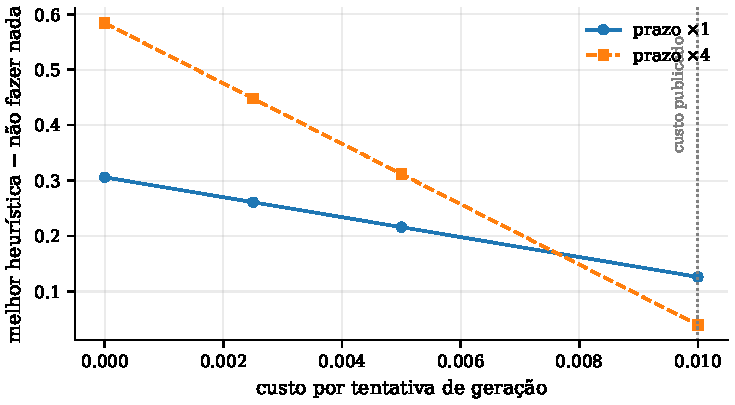
\includegraphics{figs/custo-tentativa.pdf}
\caption{O prêmio que resta para o aprendiz: melhor heurística menos a política
de não fazer nada. A curva do prazo quádruplo cruza para perto de zero
exatamente no custo por tentativa que o ambiente cobrava.}
\label{fig:custotentativa}
\end{figure}

Tornando a cobrança invariante ao prazo, o prêmio volta a 0,448 e três de três
sementes passam a treinar, contra uma de três antes. Ainda assim, a melhor
semente fica em $-0{,}012 \pm 0{,}014$ contra a heurística gananciosa, pareado
por requisição: um empate. A conclusão é que o regime de prazo longo com
heralding caro \emph{não tem decisão de temporização que valha} --- a geração
domina o orçamento e tomar a maior fidelidade disponível já está perto do
ótimo. O agente aprendido não é melhor que a heurística aqui, e o artigo não o
apresenta como se fosse.

\subsection{Alocação híbrida}

Cobrando o custo de bloco finito, o serviço de chave de todas as políticas cai
entre 30\% e 55\%, sem alterar a ordenação --- mas movendo o ponto de operação,
porque um controlador que paga o preço real da chave compra menos vazão
clássica. Por isso as fronteiras foram retraçadas em vez de a conclusão ser
extrapolada, e ela sobrevive: a serviço de chave igualado, dentro da
sobreposição das duas fronteiras, o alocador preditivo entrega
\textbf{2,7$\times$} a vazão clássica da admissão estática, contra 2,4$\times$
medidos com chave assintótica.

A Figura~\ref{fig:chavefinita} mostra a forma da penalidade de bloco finito por
compensador. Para os preditores, blocos de dez segundos recuperam 80\% do
assintótico; para a persistência, nenhuma duração recupera mais que 3\%, e a
partir de cinco segundos a curva encosta em zero --- um enlace que a fórmula
assintótica descrevia como produzindo 17 kbit/s.

\begin{figure}[ht]
\centering
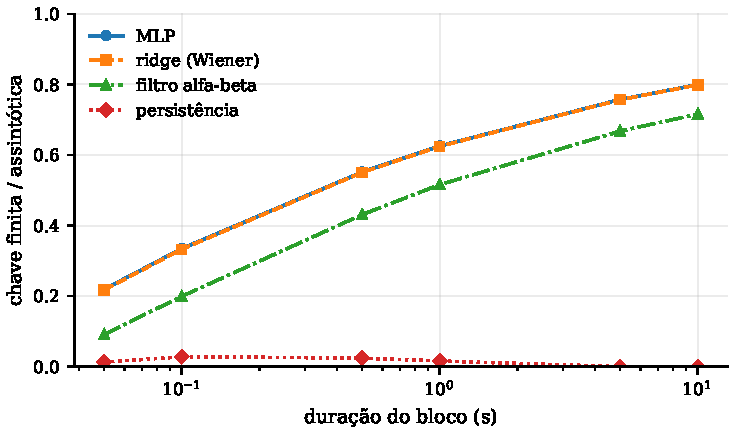
\includegraphics{figs/chave-finita.pdf}
\caption{Fração da taxa assintótica que sobrevive ao limite de chave finita,
por duração de bloco. A penalidade não é um fator comum: ela cresce conforme a
QBER se aproxima do limiar, e o compensador pior desaparece.}
\label{fig:chavefinita}
\end{figure}

\subsection{Blocagem de chave de duração variável}

A Tabela~\ref{tab:blocos} compara as estratégias da Seção 5.4 em 12 sementes de
teste, com a chave sempre dividida pela execução inteira --- descartar tempo,
portanto, nunca maquia o resultado.

\begin{table}[ht]
\caption{Blocagem de chave, 12 sementes de teste. ``Melhor fixo'' é o melhor
temporizador escolhido com retrospectiva, por compensador.}
\label{tab:blocos}
\centering
\small
\begin{tabular}{lrrrrr}
\toprule
compensador & QBER & melhor fixo & fixo 1 s & controlador & oráculo \\
            &      & (bit/s)     & (bit/s)  & agrupado (bit/s) & agrupado (bit/s) \\
\midrule
persistência     & 0,134 & 518 (0,1 s)     & 212     & \textbf{4075} & 4299 \\
filtro alfa-beta & 0,039 & 39\,987 (20 s)  & 27\,217 & 39\,295       & 40\,352 \\
ridge (Wiener)   & 0,007 & 73\,029 (20 s)  & 54\,776 & 72\,689       & 73\,109 \\
MLP              & 0,007 & 73\,520 (20 s)  & 55\,188 & 73\,171       & 73\,593 \\
\bottomrule
\end{tabular}
\end{table}

No enlace mal compensado, \textbf{temporizador de cinco segundos ou mais produz
zero bits}, de qualquer duração, em todas as doze sementes. O controlador
agrupado entrega 4075 bit/s --- 7,9$\times$ o melhor temporizador e 95\% do seu
oráculo --- montando \emph{um} bloco com cerca de 29 pedaços, 28\% da execução ao
todo: as janelas boas espalhadas por vinte segundos, liquidadas juntas. O
oráculo por intervalos, que não pode fazer isso, para em 1305 bit/s. Nos
compensadores bons o melhor bloco é um só, do tamanho da execução, e o
controlador o encontra sozinho ao custo de menos de 1\%.

A objeção óbvia é que ninguém opera com a persistência. A
Tabela~\ref{tab:stress} e a Figura~\ref{fig:blocagem} repetem a comparação no
melhor compensador, com a amplitude de vibração subindo.

\begin{table}[ht]
\caption{Blocagem sob perturbação crescente, no melhor compensador (MLP),
6 sementes por ponto.}
\label{tab:stress}
\centering
\small
\begin{tabular}{lrrrrr}
\toprule
amplitude & QBER & melhor fixo & fixo 1 s & agrupado & sobre o melhor fixo \\
\midrule
0,3 rad & 0,008 & 72\,781 & 54\,576 & 72\,092 & 0,99$\times$ \\
0,6 rad & 0,051 & 29\,914 & 21\,792 & 41\,446 & \textbf{1,39}$\times$ \\
0,9 rad & 0,202 & 2\,110  & 401     & 6\,814  & \textbf{3,23}$\times$ \\
1,2 rad & 0,322 & 314     & \textbf{0} & 876  & \textbf{2,79}$\times$ \\
\bottomrule
\end{tabular}
\end{table}

\begin{figure}[ht]
\centering
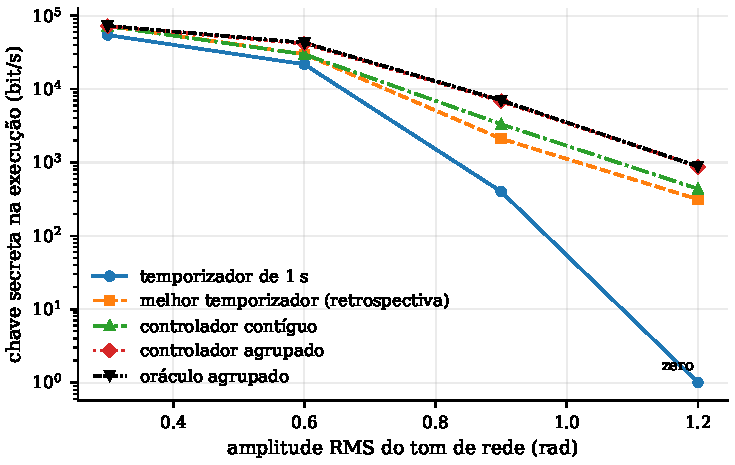
\includegraphics{figs/blocagem.pdf}
\caption{Quem escolhe o fim do bloco, no melhor compensador, à medida que o
enlace piora. Escala logarítmica, com o zero rebaixado a 1 bit/s para caber. As
curvas se separam onde o enlace deixa de ser estacionário o bastante para uma
duração só estar certa.}
\label{fig:blocagem}
\end{figure}

Abaixo do ponto de operação nominal o controlador custa 1\% e não serve para
nada. A partir do dobro da amplitude ele bate o melhor temporizador
\emph{escolhido com retrospectiva} por 1,4 a 3,2$\times$, enquanto o
temporizador de um segundo entrega zero na ponta, e fica entre 97\% e 99\% do
seu oráculo em toda a varredura.

A regra míope óbvia --- encerrar quando o segmento novo derrubaria a chave
estimada do bloco --- foi implementada primeiro e é mensuravelmente pior:
encerra em cima do ruído da estimativa, corta o enlace bom em blocos de dois
segundos onde havia vinte disponíveis, e entrega cerca de um quinto a menos de
chave. Comparar o momento com o momento seguinte não basta; é preciso comparar
dois futuros.

\subsection{Generalização em frequência: o segundo resultado negativo}

Um compensador por enlace exige um polarímetro e uma corrida de treino por
enlace, o que é um produto muito diferente de um modelo único. A pergunta é se
um modelo cobre a faixa de frequências plausíveis. Ele não cobre.

Um modelo treinado sobre 45--180 Hz e testado em cinco tons retidos fica em QBER
média 0,0615 com janela longa densa e 0,0793 com a janela curta original ---
ambos \emph{piores} que o filtro alfa-beta clássico (0,0480) e 2,4 a
3,1$\times$ o especialista treinado na frequência certa (0,0252). A dispersão
entre três inicializações é no máximo 0,0057, quase uma ordem abaixo das
diferenças, de modo que a ordenação é real.

Duas hipóteses de correção foram testadas e ambas falharam. Alongar a janela de
observação de 32 para 126 ms ajuda (0,079 para 0,062) e não basta. Fornecer a
frequência estimada como entrada explícita --- um escalar causal obtido da
recorrência que uma oscilação pura satisfaz,
$x[k+1] + x[k-1] = 2\cos(\omega\Delta t)\,x[k]$, ajustada por mínimos quadrados
sobre a primeira diferença da própria janela --- \emph{piora} as duas janelas,
reprodutivelmente. O achado útil é lateral: um conjunto de atrasos
\emph{diluído} (1, 2, 3, 4, 6, 8, 11, 16, 22, 32, 45, 63 passos) alcança os
mesmos 126 ms com 39 características contra 192 da janela densa, e empata com
ela.

\begin{figure}[ht]
\centering
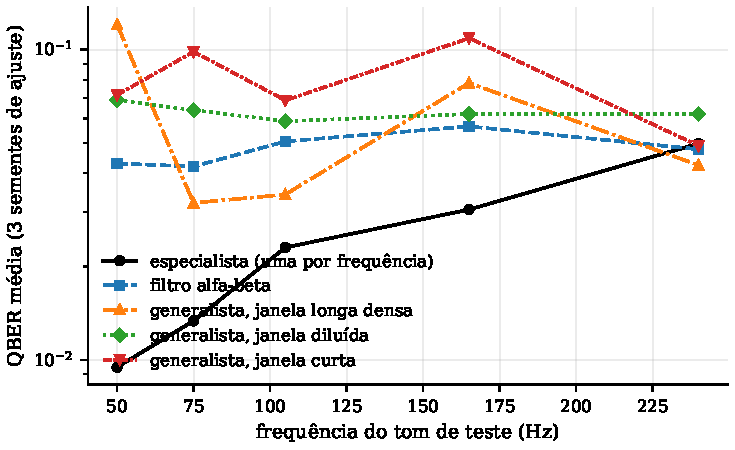
\includegraphics{figs/condicionamento.pdf}
\caption{Um modelo só sobre 45--180 Hz, por tom retido. A média da banda
esconde dois modos de falha: a janela longa densa chega perto do especialista
em 75 e 105 Hz e desaba em 50 Hz --- que fica \emph{entre} dois dos seus
próprios pontos de treino; a diluída é plana e medíocre em toda a banda.}
\label{fig:condicionamento}
\end{figure}

A Figura~\ref{fig:condicionamento} mostra por que três inicializações eram
necessárias: os dois modos de falha têm médias parecidas e dispersões pequenas
demais para serem azar de inicialização. É também aqui, e só aqui, que a rede
neural bate o ridge --- uma \emph{mistura} de frequências não é um processo
gaussiano estacionário, e o preditor precisa inferir qual tom está vendo antes
de prever a fase dele, o que não é função linear da janela. O achado negativo
das seções anteriores não estava errado; estava restrito a tarefas com um
regime só.

A recomendação que sobrevive é uma família de modelos por faixa estreita com um
seletor, agora com a alternativa eliminada em vez de apenas não tentada.

% ---------------------------------------------------------------------------
\section{Três Parâmetros que a Avaliação Corrigiu}

As três subseções seguintes descrevem premissas do sistema que a metodologia da
Seção 6 mostrou estarem erradas. São relatadas porque cada uma mudou um número
publicado e porque nenhuma delas apareceria em qualquer teste rodando dentro do
mesmo ambiente.

\subsection{O custo temporal de uma tentativa de heralding}

O ambiente analítico cobrava \emph{uma} travessia do vão por tentativa de
heralding --- o tempo de voo do fóton até o ponto médio e o retorno do aviso. O
protocolo do simulador cobra \textbf{4,1}, porque uma tentativa é uma
negociação de várias mensagens. A Figura~\ref{fig:custoheralding} mostra que a
razão é constante ao longo de um fator de oito em distância: uma sobrecarga
aditiva encolheria como fração da rodada conforme o vão cresce, e esta não
encolhe.

\begin{figure}[ht]
\centering
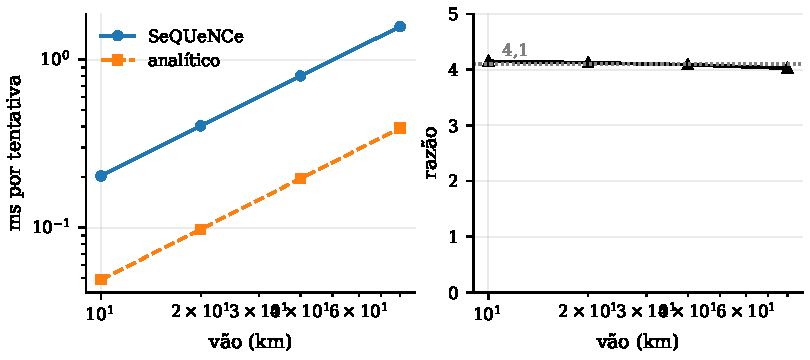
\includegraphics{figs/custo-heralding.pdf}
\caption{Custo temporal de uma tentativa de heralding. À esquerda, os dois
simuladores; à direita, a razão entre eles, estável em 4,1 ao longo de um fator
de oito em distância.}
\label{fig:custoheralding}
\end{figure}

Corrigido o custo, a vantagem de roteamento que o pacote havia medido com o
custo antigo desaparece e o agente passa a empatar com as heurísticas, como
reporta a Seção 7.2. O parâmetro estava no ambiente de treino \emph{e} no de
teste, de modo que nenhuma avaliação interna poderia tê-lo revelado.

\subsection{A cobrança por tentativa não é invariante ao prazo}

O segundo é a assimetria descrita na Seção 7.2: custo por tentativa fixo contra
custo de tempo proporcional ao prazo. A consequência de método é geral e vale
para qualquer varredura de prazo neste ambiente --- a recompensa muda de
significado junto com o prazo, e duas varreduras comparadas entre si estão
comparando duas tarefas diferentes.

\subsection{A banda mecânica e a taxa de deriva}

A banda mecânica havia sido posta em 40 Hz por plausibilidade. Nada medido
sustenta esse valor: a única polarimetria a 4 kHz publicada em fibra aérea
reporta um tom na frequência da rede elétrica com harmônicos em 120 e 180 Hz
\cite{peterson2004}, porque a fibra está dentro do cabo para-raios de uma linha
de transmissão e é a corrente nesse condutor que a move. O compensador treinado
em 40 Hz, avaliado no ponto calibrado, é \emph{pior que não compensar}. A taxa
de deriva também estava rápida demais: o expoente espectral medido,
$\beta = 1{,}0 \pm 0{,}2$ \cite{ramaswamy2026}, é função sensível da taxa neste
modelo e fixa-a entre 0,015 e 0,020 rad/s, contra os 0,05 supostos. Os
resultados da Seção 7 são todos posteriores a essa recalibração.

\subsection{Dois parâmetros que o simulador descarta em silêncio}

O mesmo programa de confronto encontrou dois parâmetros que o SeQUeNCe 1.0.0
aceita e ignora. O primeiro é a fidelidade de porta. O segundo é mais sutil:
o método que atualiza os parâmetros de um arranjo de memórias
(\texttt{update\_memory\_params}) é um \texttt{setattr} nu, e a taxa de
decoerência é derivada do tempo de coerência apenas no construtor --- ajustar o tempo de coerência depois não decoere nada, e toda
fidelidade da execução passa a ser a bruta. Ambos produzem resultados
otimistas e nenhum dos dois levanta erro.

% ---------------------------------------------------------------------------
\section{Limitações}

\textbf{Não há série temporal de fibra real.} A calibração usa estatísticas
publicadas, não gravações. A amplitude do tom da rede elétrica em particular não
está medida em nenhuma fonte acessível; uma varredura de fator 50 mostra que a
escolha entre compensadores não depende dela, mas quanta chave o enlace produz
depende.

\textbf{O bloco não contíguo não foi levado ao protocolo.} A Seção 7.4 modela a
contabilidade --- bits e taxa de erro. A sinalização não está modelada: as duas
pontas precisam concordar sobre quais índices entram no bloco, e essa lista é
tráfego clássico autenticado que não foi dimensionado aqui. Ela é pequena
(intervalos, não bits) e a reconciliação de erros já publica muito mais, mas
isso é um argumento, não uma medida.

\textbf{O motor de regras do simulador continua fora.} O executor de eventos
dirige os protocolos diretamente, porque o objetivo era pôr uma política
aprendida no lugar da política do simulador. Contenção entre requisições
concorrentes segue sem teste.

\textbf{Uma topologia de treino.} O agente é treinado numa cadeia de quatro nós
e testado em topologias não vistas, mas não sobre uma \emph{distribuição} de
topologias.

\textbf{Um ponto de operação por medida.} O cruzamento de velocidade de atuador
entre 120 e 250 rad/s é propriedade daquela banda acústica e daquela latência,
não uma constante.

% ---------------------------------------------------------------------------
\section{Conclusão}

O \texttt{qnet\_autopilot} implementa quatro capacidades de controle aprendido
para redes quânticas sobre uma camada de física conferida contra um simulador
de eventos discretos estabelecido, e mede cada uma contra a melhor alternativa
simples disponível, ressintonizada.

Duas das quatro entregam vantagem. O compensador de polarização reduz a QBER de
0,0383 --- melhor filtro clássico ressintonizado --- para 0,0074, com a condição
de hardware explícita de um atuador acima de 250 rad/s. O alocador preditivo
entrega 2,7$\times$ a vazão clássica da admissão estática a serviço de chave
igualado, e a conclusão sobrevive à contabilidade de chave finita.

A terceira é o resultado mais forte do trabalho e não é uma rede neural: o
controlador causal de bloco de chave, sem constante de ajuste, decide onde
cortar os blocos a partir das mesmas estimativas ruidosas que o protocolo já
publica, e entrega chave onde temporizador nenhum entrega bit algum --- 4075
bit/s contra zero --- ao custo de 1\% onde o enlace é fácil. O mecanismo que o
torna possível é uma leitura do limite de chave finita, não do modelo: a chave
de um bloco não depende de quando os bits chegaram, de modo que um receptor
pode liquidar janelas boas separadas como um bloco só.

A quarta não entrega vantagem, e o motivo é informativo: com o custo de
heralding medido, o regime em que o agente de roteamento operaria não tem
decisão de temporização que valha, porque a geração domina o orçamento. Junto
com a impossibilidade medida de cobrir 45--180 Hz com um compensador único, isso
delimita onde aprendizado ajuda neste domínio --- e onde a resposta correta é
uma heurística ou uma família de modelos estreitos.

\section*{Disponibilidade}

O pacote acompanha este artigo com 861 testes automatizados, os \emph{scripts}
que reproduzem cada tabela e os relatórios que contêm as figuras completas de
cada estudo. Todo resultado negativo descrito aqui está registrado no
código-fonte junto à rotina que o produziu.

\begin{thebibliography}{99}

\bibitem[Barrett and Kok(2005)]{barrett2005} Barrett, S. D. and Kok, P. (2005). Efficient high-fidelity quantum
computation using matter qubits and linear optics. \emph{Physical Review A},
71(6):060310(R).

\bibitem[Bennett et al.(1996)]{bennett1996} Bennett, C. H., Brassard, G., Popescu, S., Schumacher, B., Smolin,
J. A., and Wootters, W. K. (1996). Purification of noisy entanglement and
faithful teleportation via noisy channels. \emph{Physical Review Letters},
76(5):722--725. Errata: \emph{Physical Review Letters}, 78:2031 (1997).

\bibitem[Briegel et al.(1998)]{briegel1998} Briegel, H.-J., Dür, W., Cirac, J. I., and Zoller, P. (1998). Quantum
repeaters: the role of imperfect local operations in quantum communication.
\emph{Physical Review Letters}, 81(26):5932--5935.

\bibitem[Chapuran et al.(2009)]{chapuran2009} Chapuran, T. E., Toliver, P., Peters, N. A., Jackel, J., Goodman,
M. S., Runser, R. J., McNown, S. R., Dallmann, N., Hughes, R. J., McCabe,
K. P., Nordholt, J. E., Peterson, C. G., Tyagi, K. T., Mercer, L., and Dardy,
H. (2009). Optical networking for quantum key distribution and quantum
communications. \emph{New Journal of Physics}, 11:105001.

\bibitem[Chittoor and Simeone(2023)]{chittoor2023} Chittoor, H. H. S. and Simeone, O. (2023). Quantum machine learning
for distributed quantum protocols with local operations and noisy classical
communications. \emph{Entropy}, 25(2):352.

\bibitem[Czegledi et al.(2016)]{czegledi2016} Czegledi, C. B., Karlsson, M., Agrell, E., and Johannisson, P. (2016).
Polarization drift channel model for coherent fibre-optic systems.
\emph{Scientific Reports}, 6:21217.

\bibitem[Deutsch et al.(1996)]{deutsch1996} Deutsch, D., Ekert, A., Jozsa, R., Macchiavello, C., Popescu, S., and
Sanpera, A. (1996). Quantum privacy amplification and the security of quantum
cryptography over noisy channels. \emph{Physical Review Letters},
77(13):2818--2821. Errata: \emph{Physical Review Letters}, 80:2022 (1998).

\bibitem[Dynes et al.(2019)]{dynes2019} Dynes, J. F., Wonfor, A., Tam, W. W.-S., Sharpe, A. W., Takahashi, R.,
Lucamarini, M., Plews, A., Yuan, Z. L., Dixon, A. R., Cho, J., Tanizawa, Y.,
Elbers, J.-P., Greißer, H., White, I. H., Penty, R. V., and Shields, A. J.
(2019). Cambridge quantum network. \emph{npj Quantum Information}, 5:101.

\bibitem[Eraerds et al.(2010)]{eraerds2010} Eraerds, P., Walenta, N., Legré, M., Gisin, N., and Zbinden, H.
(2010). Quantum key distribution and 1 Gbps data encryption over a single
fibre. \emph{New Journal of Physics}, 12(6):063027.

\bibitem[Krastanov et al.(2019)]{krastanov2019} Krastanov, S., Albert, V. V., and Jiang, L. (2019). Optimized
entanglement purification. \emph{Quantum}, 3:123.

\bibitem[Krutyanskiy et al.(2023)]{krutyanskiy2023} Krutyanskiy, V., Canteri, M., Meraner, M., Bate, J., Krcmarsky, V.,
Schupp, J., Sangouard, N., and Lanyon, B. P. (2023). Telecom-wavelength quantum
repeater node based on a trapped-ion processor. \emph{Physical Review
Letters}, 130(21):213601.

\bibitem[Kumar et al.(2015)]{kumar2015} Kumar, R., Qin, H., and Alléaume, R. (2015). Coexistence of continuous
variable QKD with intense DWDM classical channels. \emph{New Journal of
Physics}, 17(4):043027.

\bibitem[Le and Nguyen(2022)]{le2022} Le, L. and Nguyen, T. N. (2022). Entanglement routing for quantum
networks: a deep reinforcement learning approach. In \emph{ICC 2022 --- IEEE
International Conference on Communications}, p. 395--400.

\bibitem[Mnih et al.(2016)]{mnih2016} Mnih, V., Badia, A. P., Mirza, M., Graves, A., Lillicrap, T., Harley,
T., Silver, D., and Kavukcuoglu, K. (2016). Asynchronous methods for deep
reinforcement learning. In \emph{Proceedings of the 33rd International
Conference on Machine Learning}, PMLR 48:1928--1937.

\bibitem[Ng et al.(1999)]{ng1999} Ng, A. Y., Harada, D., and Russell, S. (1999). Policy invariance under
reward transformations: theory and application to reward shaping. In
\emph{Proceedings of the 16th International Conference on Machine Learning},
p. 278--287.

\bibitem[Noé et al.(1988)]{noe1988} Noé, R., Heidrich, H., and Hoffmann, D. (1988). Endless polarization
control systems for coherent optics. \emph{Journal of Lightwave Technology},
6(7):1199--1208.

\bibitem[Peters et al.(2009)]{peters2009} Peters, N. A., Toliver, P., Chapuran, T. E., Runser, R. J., McNown,
S. R., Peterson, C. G., Rosenberg, D., Dallmann, N., Hughes, R. J., McCabe,
K. P., Nordholt, J. E., and Tyagi, K. T. (2009). Dense wavelength multiplexing
of 1550 nm QKD with strong classical channels in reconfigurable networking
environments. \emph{New Journal of Physics}, 11(4):045012.

\bibitem[Peterson et al.(2004)]{peterson2004} Peterson Jr., D. L., Leo, P. J., and Rochford, K. B. (2004). Field
measurements of state of polarization and PMD from a tier-1 carrier. In
\emph{Technical Digest, Optical Fiber Communication Conference (OFC)}, Los
Angeles.

\bibitem[Ramaswamy et al.(2026)]{ramaswamy2026} Ramaswamy, A., Rao, N. S. V., Chapman, J. C., and Alshowkan, M.
(2026). Analysis of polarization drift of optical signals over deployed
aerial-inground fiber connections. arXiv:2607.07629.

\bibitem[Rode et al.(2025)]{rode2025} Rode, A., Farsi, M., Lauinger, V., Karlsson, M., Agrell, E., Schmalen,
L., and Häger, C. (2025). Machine learning opportunities for integrated
polarization sensing and communication in optical fibers. \emph{Optical Fiber
Technology}, 90:104047.

\bibitem[Roik et al.(2024)]{roik2024} Roik, J., Bartkiewicz, K., Černoch, A., and Lemr, K. (2024). Routing
in quantum communication networks using reinforcement machine learning.
\emph{Quantum Information Processing}, 23(3):89.

\bibitem[Schulman et al.(2016)]{schulman2016} Schulman, J., Moritz, P., Levine, S., Jordan, M. I., and Abbeel, P.
(2016). High-dimensional continuous control using generalized advantage
estimation. In \emph{4th International Conference on Learning Representations
(ICLR)}. arXiv:1506.02438.

\bibitem[Shi et al.(2026)]{shi2026} Shi, Y., Su, J., Rahmouni, A., Shrestha, P., Merzouki, M., Bello
Portmann, G., Lazenby, A., Flament, M., Namazi, M., Battou, A., Slattery, O.,
and Gerrits, T. (2026). Entanglement distribution over a polarization-stabilized
aerial fiber. arXiv:2601.11753.

\bibitem[Tomamichel et al.(2012)]{tomamichel2012} Tomamichel, M., Lim, C. C. W., Gisin, N., and Renner, R. (2012). Tight
finite-key analysis for quantum cryptography. \emph{Nature Communications},
3:634.

\bibitem[Uhlenbeck and Ornstein(1930)]{uhlenbeck1930} Uhlenbeck, G. E. and Ornstein, L. S. (1930). On the theory of the
Brownian motion. \emph{Physical Review}, 36(5):823--841.

\bibitem[Wallnöfer et al.(2020)]{wallnofer2020} Wallnöfer, J., Melnikov, A. A., Dür, W., and Briegel, H. J. (2020).
Machine learning for long-distance quantum communication. \emph{PRX Quantum},
1:010301.

\bibitem[Werner(1989)]{werner1989} Werner, R. F. (1989). Quantum states with Einstein-Podolsky-Rosen
correlations admitting a hidden-variable model. \emph{Physical Review A},
40(8):4277--4281.

\bibitem[Wu et al.(2021)]{wu2021} Wu, X., Kolar, A., Chung, J., Jin, D., Zhong, T., Kettimuthu, R., and
Suchara, M. (2021). SeQUeNCe: a customizable discrete-event simulator of
quantum networks. \emph{Quantum Science and Technology}, 6(4):045027.

\bibitem[Young et al.(2026)]{young2026} Young, A., Duan, R., Pirandola, S., and Lucamarini, M. (2026). A
comparison of optimisation algorithms for electronic polarisation control in
quantum key distribution. \emph{Applied Sciences}, 16(5):2568.

\bibitem[Zhang et al.(2021)]{zhang2021} Zhang, S., Liu, J., Zeng, G., Zhang, C., Zhou, X., and Wang, Q.
(2021). Machine learning-assisted measurement device-independent quantum key
distribution on reference frame calibration. \emph{Entropy}, 23(10):1242.

\end{thebibliography}

\end{document}
